\section{Experiments}
\label{sec:exp}
In experiments, we compare our CYAN-RNN 
to the state-of-the-art modeling methods of cascade prediction on both
synthetic and real data. 
The results show that CYAN-RNN can better model cascade dynamics
and infer propagation structure.

\subsection{Baselines}
% We choose Recurrent Marked Temporal Point Process (RMTPP)~\cite{DuKDD2016} as
% one of the baselines which can models both next activated user and time based on
% RNN.
% \begin{itemize}
%   \item \textbf{RMTPP}~\cite{DuKDD2016}: Recurrent marked temporal point process
%   (RMTPP) is a method which can models both next activated user and time based on RNN.
% \end{itemize}
% However, only RMTPP~\cite{DuKDD2016} can predict next propagations completely
% including both next actived user and time. To better illustrate the performance of our
% proposed model, we choose other state-of-the-art models for either predicting
% next activated users or predicting next activated time for comparisons in two
% prediction tasks.

Rare methods can predict next propagations completely including both next
activated users and time. To better illustrate the performance of our
proposed model, we choose the state-of-the-art modeling methods for either
predicting next activated users or predicting next activated time for comparisons in two
prediction tasks.

(1) Prediction of next activated user
\begin{itemize}
  \item \textbf{CT Bernoulli} and \textbf{CT Jaccard}
  models~\cite{goyal2010learning}: They are continuous time propagation models.
  The propagation probabilities between two users are defined by Bernoulli or
  Jaccard distribution and the probabilities are decayed over time.
  \item \textbf{MC-1} Model: The markov chain model is a classic sequence
  modeling method. Here we compare with markov chain with order one.
\end{itemize}

(2) Prediction of next activated time 
\begin{itemize}
  \item \textbf{Poisson process} model~\cite{vere1988introduction}: It is a
  stoachastic point process model, depicting the time consuming from one
  propagation to another. The intensity function is parameterized by a constant.
  \item \textbf{Hawkes process} model~\cite{hawkes1971spectra}: It is a
  stochastic point process model where the intensity function is parameterized by
  \begin{equation} 
  \label{eq:hawke_intens_func}
  \lambda(t)=\lambda(0)+\alpha\sum_{t_i<t}\exp\left(-\frac{t-t_i}{\sigma}\right),
  \end{equation}
  where $\sigma=1$ and $\lambda(0)$ is a intrinsic rate when $t=0$.
\end{itemize}

We also compare with the model that has the ability to generate both mark and
temporal sequences.
\begin{itemize}
  \item \textbf{RMTPP}~\cite{DuKDD2016}: Recurrent marked temporal point process
  (RMTPP) is a method which can models both next activated user and time based on RNN.
\end{itemize}

\subsection{Synthetic Data and Results Anlaysis}
The goal of the experiments on synthetic
data is to understand how the underlying network structure and propagation
model affect our proposed model on both cascade prediction and
dependency structure inference. 

\noindent{\textbf{Data generation}} 
We use Kroneck
generator~\cite{LeskovecICML07} to construct two types of networks with directed
edges: 1) the Core-Periphery (CP) network~\cite{LeskovecWWW08} (Kroneck
parameter matrix $[0.962, 0.535; 0.535, 0.107]$), mimicing real-world social networks; 2) the
Erd\H{o}s-R{\'e}nyi random (Random) network~\cite{Erdos60} ($[0.5, 0.5; 0.5, 0.5]$). The incubation time
of one user activating anther user are sampled from the two distributions: 1)
mixed exponential (Exp) distributions, controlled by rate parameters $\alpha$
in $[0.01, 10]$; 2) mixed rayleigh (Ray) distribution, controlled
by scale parameters $\beta$ in $[0.01, 10]$. To generate a
cascade, we randomly choose a root user as the source of the cascade at first.
For each neighbor of the activated user, its activated time is determined by
incubation time. The propagation process will further conitune  in
breadth-first fashion until the overall time exceed the predefined observation
time window or no new user being activated. In our experiments, we set the total
number of users $|U|=32$ and the maximal observation time $\max\{t\}=100$.
As a result, four kinds of datasets are obtained by the different unions between
network and cascade generation distribution, denoted by (CP, Exp), (CP, Ray),
(Random, Exp) and (Random, Ray). We generate up to
20,000 cascades in each dataset, where we randomly pick up 80\% of completed sequences for training and the rest are
 evenly split into validation and test sets. 
% The policy of seperating dataset is uniform in real data.

\begin{figure*}[ht!]
\centering
\subfigure[CP, Exp] {
\label{fig:pred_usr_toy_cp_exp}
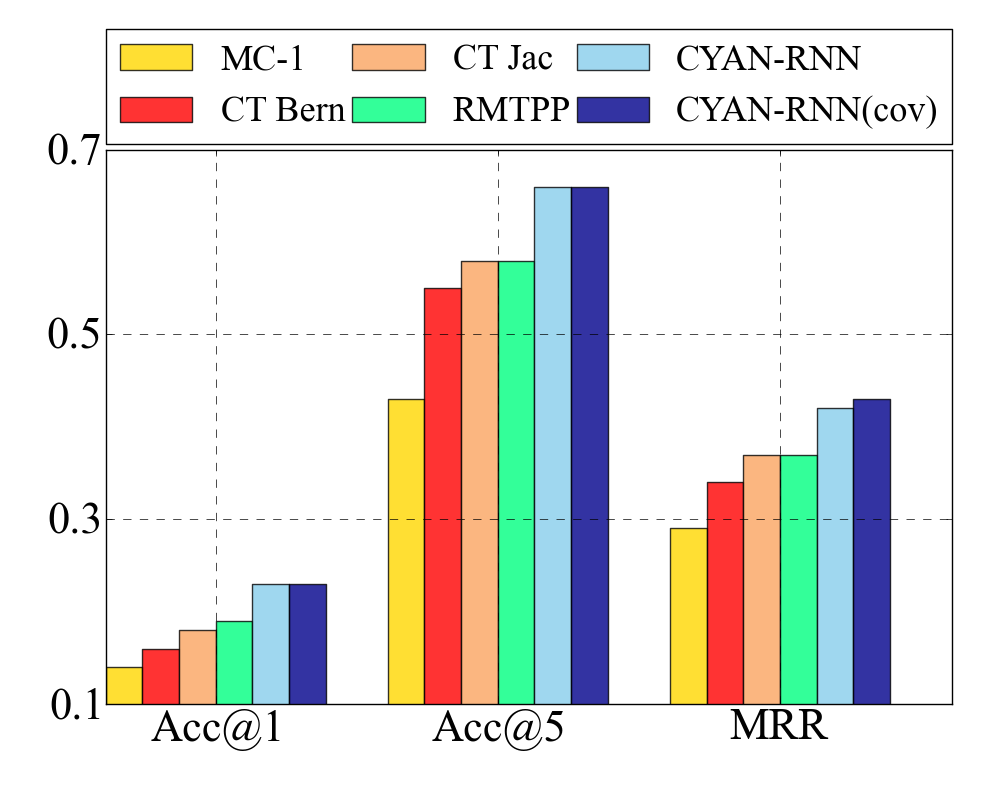
\includegraphics[width=0.235\textwidth]{figs/toy_mrr-cp-exp.png}
}
\subfigure[CP, Rayleign] {
\label{fig:pred_usr_toy_cp_ray}
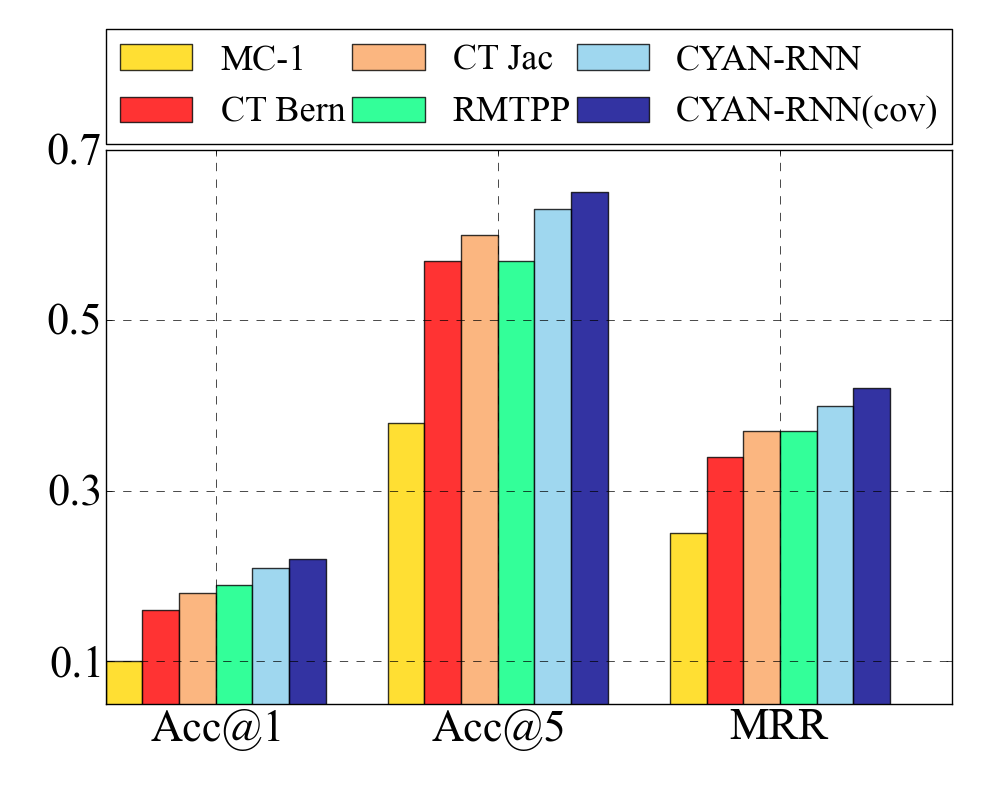
\includegraphics[width=0.235\textwidth]{figs/toy_mrr-cp-ray.png}
}
\subfigure[Random, Exp] {
\label{fig:pred_usr_toy_rand_exp}
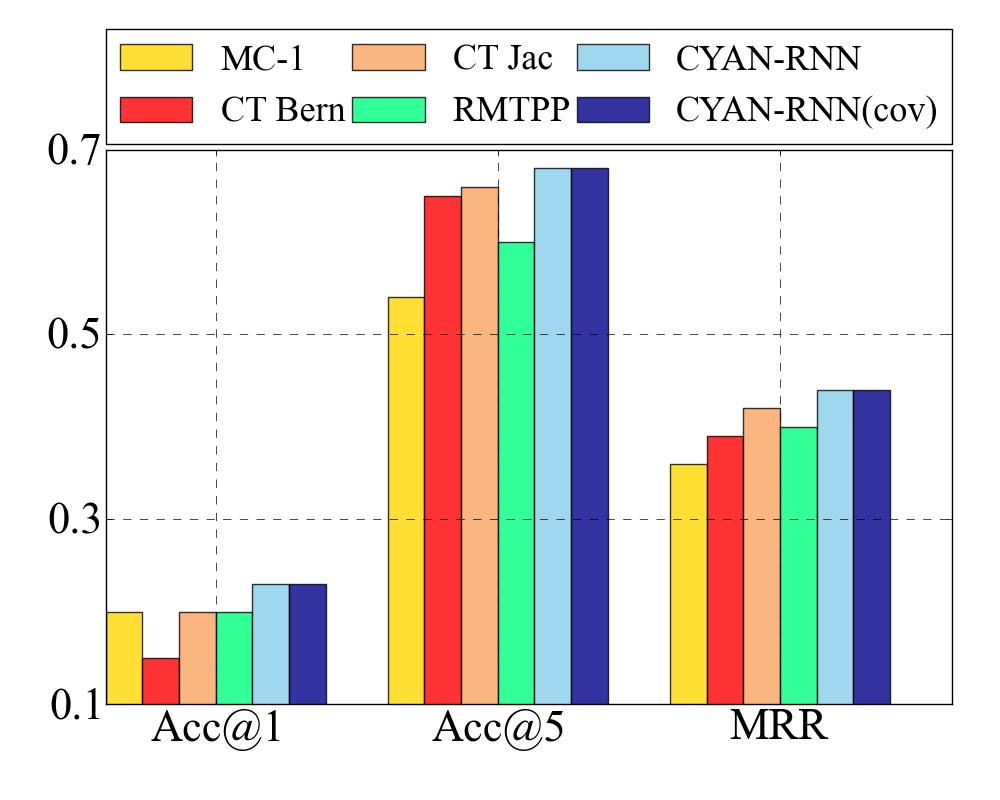
\includegraphics[width=0.235\textwidth]{figs/toy_mrr-rand-exp.png}
}
\subfigure[Random, Rayleign] {
\label{fig:pred_usr_toy_rand_ray}
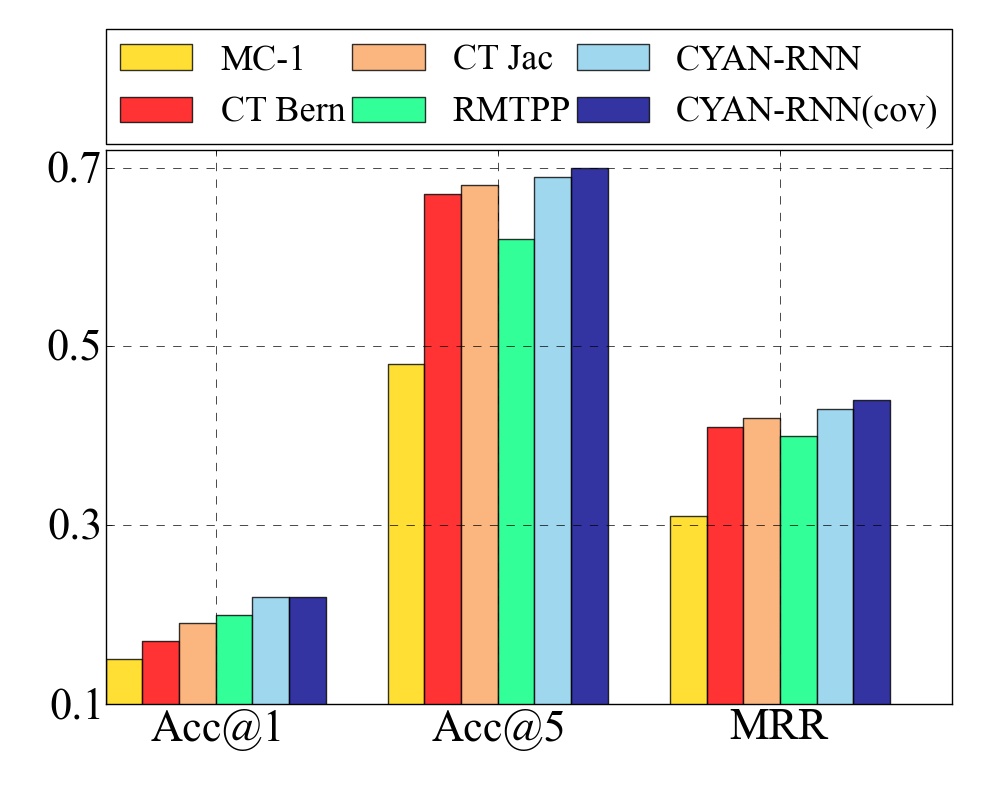
\includegraphics[width=0.235\textwidth]{figs/toy_mrr-rand-ray.png}
}
\subfigure[RMSE on toy data] {
\label{fig:pred_tm_toy_rmse}
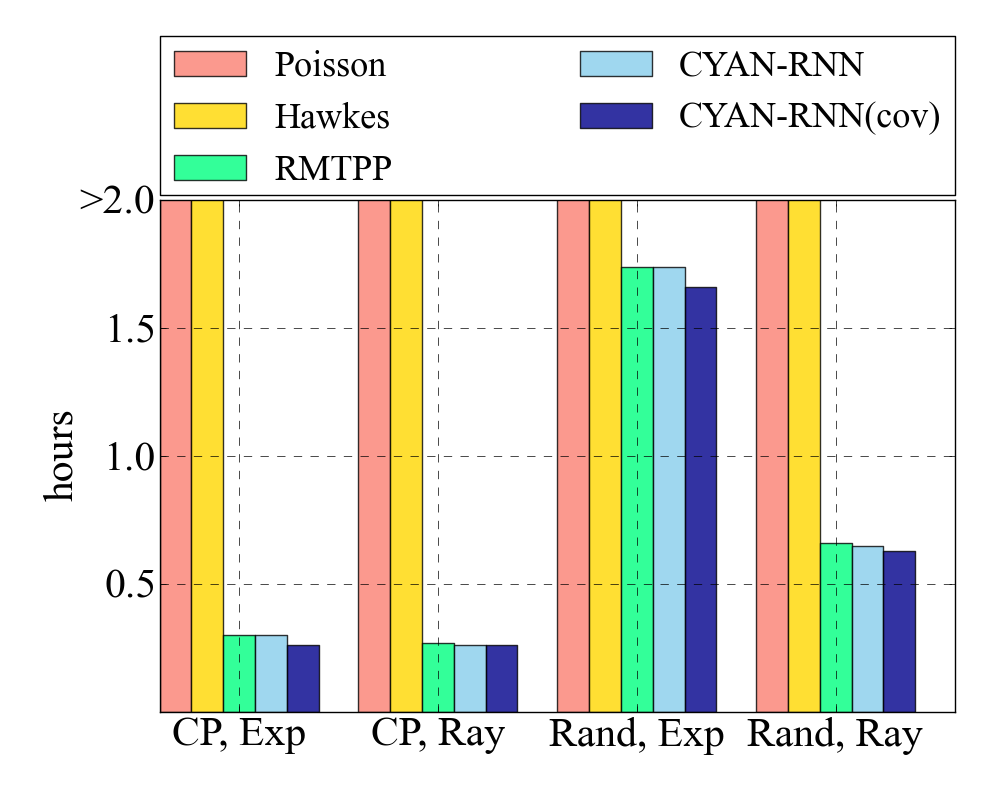
\includegraphics[width=0.235\textwidth]{figs/toy_rmse.png}
}
\subfigure[Real data] {
\label{fig:pred_usr_real}
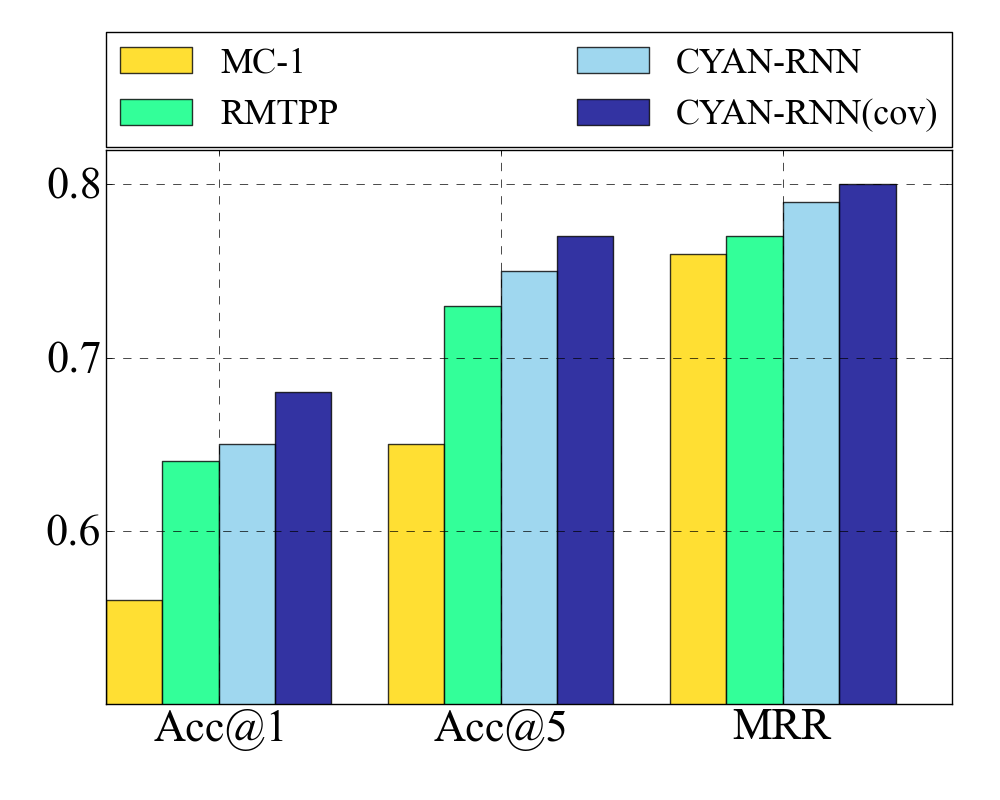
\includegraphics[width=0.235\textwidth]{figs/real_mrr.png}
}
\subfigure[RMSE on real data] {
\label{fig:pred_tm_real_rmse}
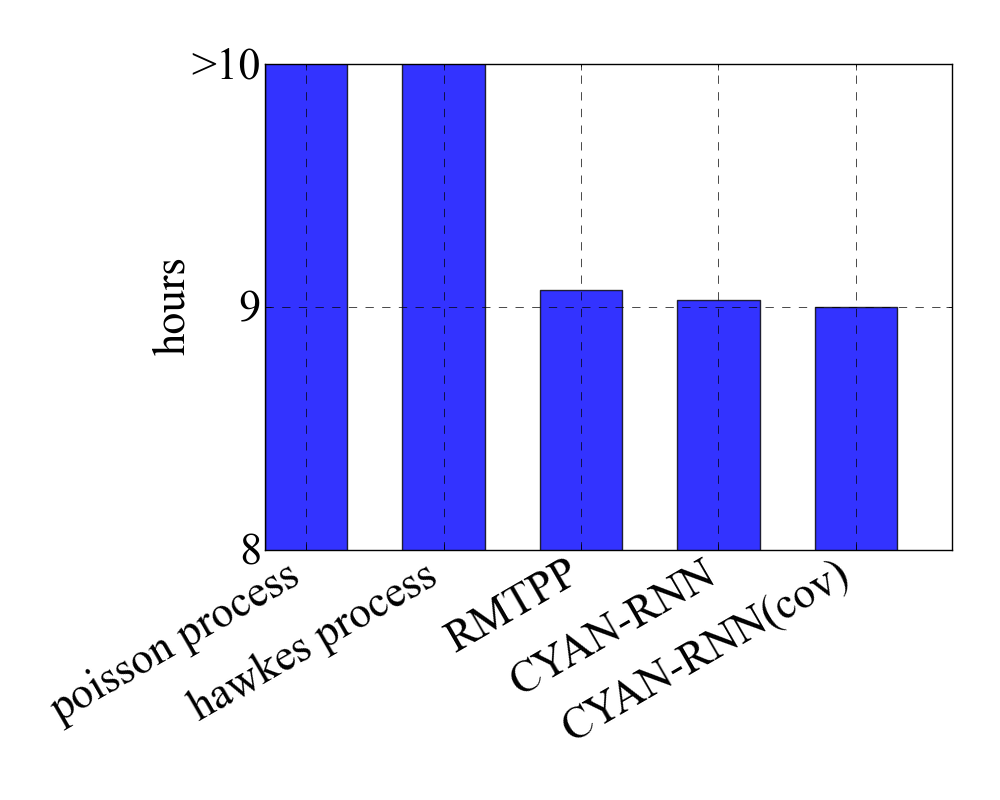
\includegraphics[width=0.235\textwidth]{figs/real_rmse.png}
}

\caption{Comparisons on baselines and our proposed models. (a)$\sim$(e) The
predictions of next activated user and time on toy data produced
from different networks and propagation models; (f) and (g) The predictions of
next activated user and time on real data.}
\end{figure*}

%\noindent{\textbf{Evaluation metrics}} 
We regard the prediction task on next activated user as a ranking problem
with respect to transition probabilities. The predictive performance is
evaluated by \textit{Accuracy on top} $k$ (Acc@$k$) and \textit{Mean Reciprocal Rank}
(MRR)~\cite{voorhees1999trec}.
% , functionized in top $k$ and global perspectives.
The larger values in Acc@$k$ and MRR indicate the better performance.
On the prediction of next activated time, we use Root Mean Square Deviation
(RMSE) between estimated time and practical occuring time. The better
performance means the small values in RMSE.   

\noindent{\textbf{Prediction results.}} 
We regard the prediction task on next activated user as a ranking problem
with respect to transition probabilities. The predictive performance is
evaluated by \textit{Accuracy on top} $k$ (Acc@$k$) and \textit{Mean Reciprocal Rank}
(MRR)~\cite{voorhees1999trec}.
% , functionized in top $k$ and global perspectives.
The larger values in Acc@$k$ and MRR indicate the better performance.
On the prediction of next activated time, we use Root Mean Square Deviation
(RMSE) between estimated time and practical occuring time. The better
performance means the small values in RMSE.   

We conduct experiments on all four
kinds of datasets. 
We firstly compare the predictive preformance on
next activated users. The results on predictions of next
activated users are shown in Fig.~\ref{fig:pred_usr_toy_cp_exp}$\sim$
\ref{fig:pred_usr_toy_rand_ray}. As shown in the figures, CYAN-RNN and CYAN-RNN(cov)
perform consistently and significantly better than other baselines in metrics of
Acc@1, Acc@5 and MRR, included in all datasets. 
% In Acc@10, our proposed models
% outperform other baselines except the cases in dataset of
% (Random, Exp). 
% Despite of this, 
The results indicate that our proposed methods can better predict next activated
users. It is interested that RMTPP has lower accuracy or MRR values than CT Bern
and CT Jac in some cases shown in
Fig.~\ref{fig:pred_usr_toy_cp_ray},
\ref{fig:pred_usr_toy_rand_exp} and \ref{fig:pred_usr_toy_rand_ray}, however,
CYAN-RNN and CYAN-RNN(cov) can still performs better. It clearly demonstrates
that the proposed attention mechanism has the ability to directly capture past
propagation information which may be ``forgetten'' by sequential transitions in
RNN, called crossing dependency problems in CDM.
% Interestingly, we can find out that the RMTPP has lower accurary or MRR
% values in datasets of (CP, Rayleign), (Random, Exp) and (Random, Rayleign).
Fig.~\ref{fig:pred_tm_toy_rmse} compares the predictive performance on RMSE.
We can observe that Poisson and Hawkes processes are the worst modeling methods,
obtaining the errors larger than 2 hours in all datasets. Meanwhile, the
RMSE values are similar between RMTPP and CYAN-RNN. But 
CYAN-RNN(cov) can perform slightly better than RMTPP and CYAN-RNN in all
datasets when predicting next activated time. 
Additionally, we can observe that CYAN-RNN(cov) consistently perform better or
even than CYAN-RNN in two prediction tasks. It indicates that the coverage can
help to efficiently utilize the propagation embeddings in attention mechanism.
Next we will exploit the answers how the coverage can help to boost predictive
performance and lead to better inference on dependency structure.

\begin{figure}
\centering
\subfigure[] {
\label{fig:cyan_deps}
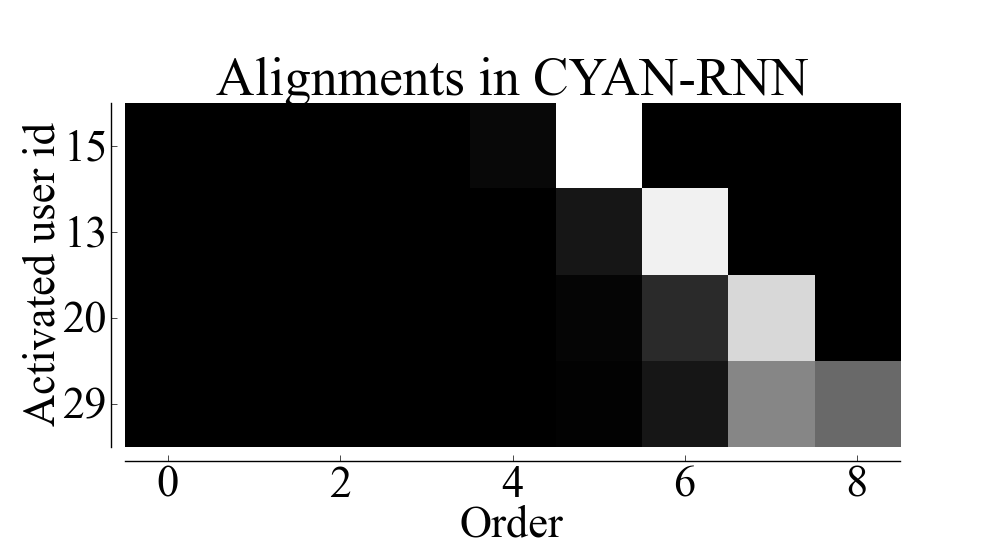
\includegraphics[width=0.225\textwidth]{figs/case_align-att.png}
}
\subfigure[] {
\label{fig:cyan_cov_deps}
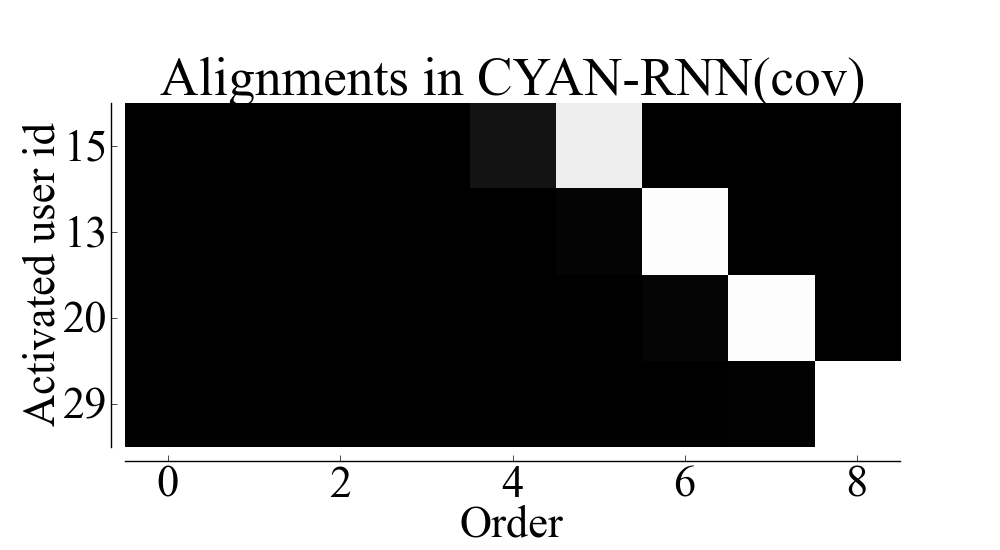
\includegraphics[width=0.225\textwidth]{figs/case_align-cov.png}
}
\caption{Sample alignments on a fragement of cascade. The y-axis is the users
who will be activated next sequentiallly from top to bottom. The x-axis is the
activated order related to next activated user in the cascade. Each pixel shows
the weight $\alpha_{k,i}$ related to $i$-th propagation embedding at each step
$k$, in grayscale (0:black, 1:white). (a) the alignments inferred by CYAN-RNN; (b) the
alignments inferred by CYAN-RNN(cov).
% the inferred Graphs of
% propagations inferred by proposed models.
% The grey lines are the ground truth of propagation paths, while the read lines are wrong
% estimations, including missing or false answers. (a) Graph of propagation
% inferred by CYAN-RNN; (b) Graph of propagation inferred by CYAN-RNN (cov). 
}
\end{figure}

\noindent{\textbf{Alignment accurary.}} 
We expect to check if coverage can reduce the over-dependence and
under-dependence mentioned in section~\ref{sec:coverage}.
Fig.~\ref{fig:cyan_deps} and \ref{fig:cyan_cov_deps} show the results. Every grid
in each plot represents the alignment weights associated with propagation
embeddings.
The brighter grid refers to the larger weights corresponding to next
propagation. From this we see which positions in the past propagations
were considered more important when predicting next propagation. Comparing to
the alignments in CYAN-RNN, we can observe that the alignments in CYAN-RNN(cov)
concentrate more on unused propagation embeddings, which is consistent to
well-studied phenomonen in published works~\cite{}. Moreover, we wonder if the
inferred alignments is homologous to true propagation structures. Thus, we
calculate alignments on each step of cascades in test data. We suggest that the
propagation structure of next propagation can be inferred by the largest
alignment at each step. We then get a matrix of statistic results based on all inferred
structures. Every column in the matrix refers to the number of who mainly
activate the propagation. As the high connection between propagation
structure and network, the inferred structures would be the edges in
network. Therefore, we normalize the matrix by rows, and check if the
network edges can be classified by the matrix. As the
inference results are same in other two datasets, we only show the AUC values
computed by the models trained in dataset of (CP, Exp) and (Random, Exp),
decribed in Table~\ref{t:auc_net_inf}. The results from our proposed models
are both worked in network inference. Besides, CYAN-RNN(cov) obtain better results of
network inference than CYAN-RNN in two test data. It indicates that our
proposed alignment mechanism can be natually used in inference of hidden
propagation structure, which may have some potential applications in practice,
e.g., advertisement and recommendation.

%  to specific user. normalized
% normalize the  and treat the ms into a classification task.
% We suppose that the
% next propagation is only related to corresponding historical propagation which
% has the largest alignment weight. As the reason of relationship
% between propagation structures and network, we expect the connection between
% next propagation and corresponding 


\begin{table}[h!]
\centering
\caption{AUC values of network inference.}
\begin{tabular*}{.38\textwidth}{c|cc} \hline
Network & CYAN-RNN & CYAN-RNN(cov) \\ \hline
CP & 0.83 & 0.84 \\
Random & 0.95 & 0.96 \\ \hline
\end{tabular*}
\label{t:auc_net_inf}
\end{table}

% \begin{table}[h]
% \centering
% \caption{Distribution of dependency on relative position (inferred vs. ground
% truth).}
% \resizebox{0.47\textwidth}{!}{
% \begin{tabular}{crcc|c} \hline
% & & CYAN-RNN & CYAN-RNN(cov) & Ground truth \\ \hline 
% \multirow{5}{*}{CP} & 1st pos & 0.005 & & 0.022 \\
%  & last pos & 0.930 & 0 & 0.326 \\
%  & 1st prev pos & 0.065 & 0.968 & 0.182 \\
%  & 2nd prev pos & 0.004 & 0.032 & 0.121 \\
%  & 3rd prev pos & 0.002 & 0 & 0.087 \\ \hline
% \multirow{5}{*}{ER} & 1st pos &  & & 0.024 \\
%  & last pos pos & & & 0.387 \\
%  & 1st prev pos & & & 0.189 \\
%  & 2nd prev pos & & & 0.118 \\
%  & 3rd prev pos & & & 0.078 \\ \hline
% \end{tabular}
% }
% \end{table}

% \noindent{\textbf{Case study: alignment quality.}}

% CP, Exp(att, cov)
% Area under the ROC curve : 0.831982
% Area under the ROC curve : 0.839126
% Random, Exp(att, cov)
% Area under the ROC curve : 0.955918
% Area under the ROC curve : 0.956609

\subsection{Real Data and Result Analysis}

\noindent{\textbf{Experimental setup.}}  
The real data is extracted from Sina Weibo, a Chinese microblogging website,
spanning from June 1st, 2016 to June 30th, 2016. We focus the records in June
1st and extract users whose posting numbers are ranged in $(100,
200]$. Then we sort records according to the root
message IDs posted by the filtered users in 30 days and arrange them ascendingly
by posting time. We drop the cascades that the number of propagations is larger
than 1,000. The long length of propagations may dominate the training process,
however, rarely occurred in practice. 
%  thus ignoring the small ones.
Finally, the processed data contains 2964 users and 596,088 cascades. 
% The average number of users postings is up to 9581.76.
We use 536,240 sequences for training, 29,758 for validation and 30,005 for
testing. The task is to predict next propagation, including activated user and
time. 

\noindent{\textbf{Prediction results.}} 
The results on predictions of next
activate users and time are shown in Fig.~\ref{fig:pred_usr_real} and
\ref{fig:pred_tm_real_rmse}. The hyper-parameters of CYAN-RNN and CYAN-RNN(cov)
are setted up as following: learning rate is 0.0001; hidden layer size of
encoder is 20; hidden layer size of decoder is 10; window size is 200; coverage
size is 10; and batch size is 128. Note that we have no social
network in extracted real data, thus we cannot compare our proposed models with
CT Bern and CT Jac. CYAN-RNN and CYAN-RNN(cov) outperform the other baselines
with higher MRR values and lower RMSE values for predicting both next activated
users and time. Comparing to RMTPP, CYAN-RNN(cov) recieves 6.25\%, 5.48\% and
3.90\% relative increased performance on Acc@1, Acc@5 and MRR respectively, and
reduces 0.78\% relative errors on RMSE. Comparing to CYAN-RNN, CYAN-RNN(cov)
recieves 4.62\%, 2.67\% and 1.27\% relative increased performance on Acc@1,
Acc@5 and MRR respectively, and reduces 0.33\% relative errors on RMSE.

% \begin{figure}[ht!]
% \centering
% \subfigure[] {
% \label{fig:pred_usr_real}
% 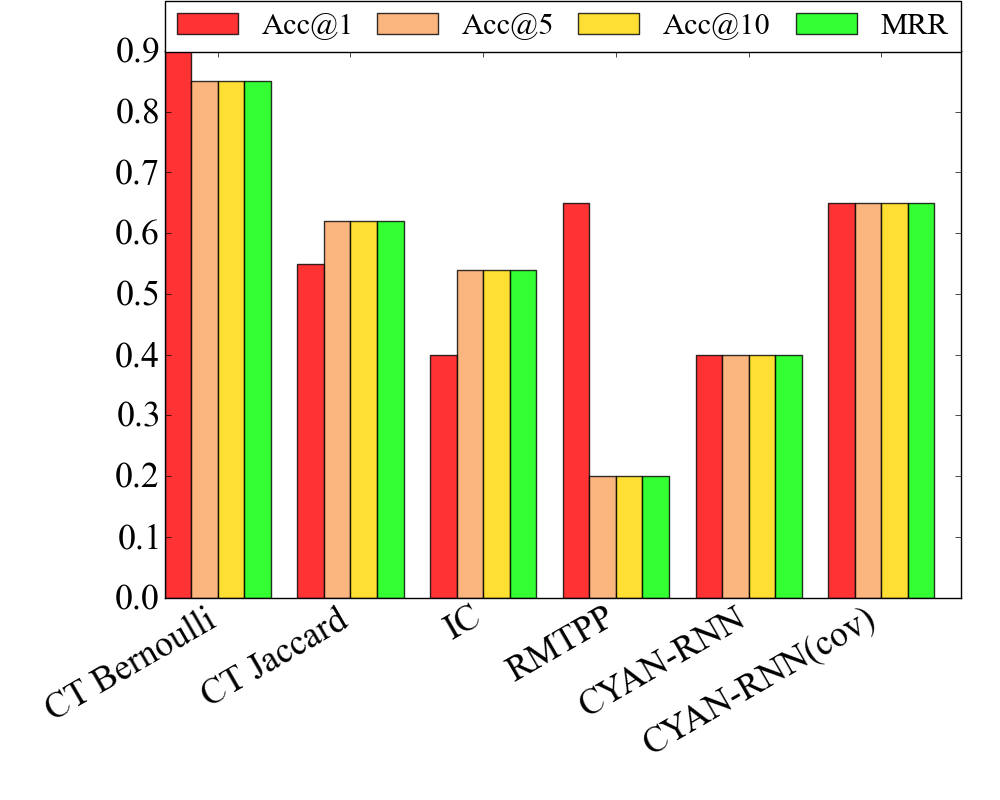
\includegraphics[width=0.35\textwidth]{figs/toy_mrr.png}
% }
% \subfigure[] {
% \label{fig:pred_tm_real}
% 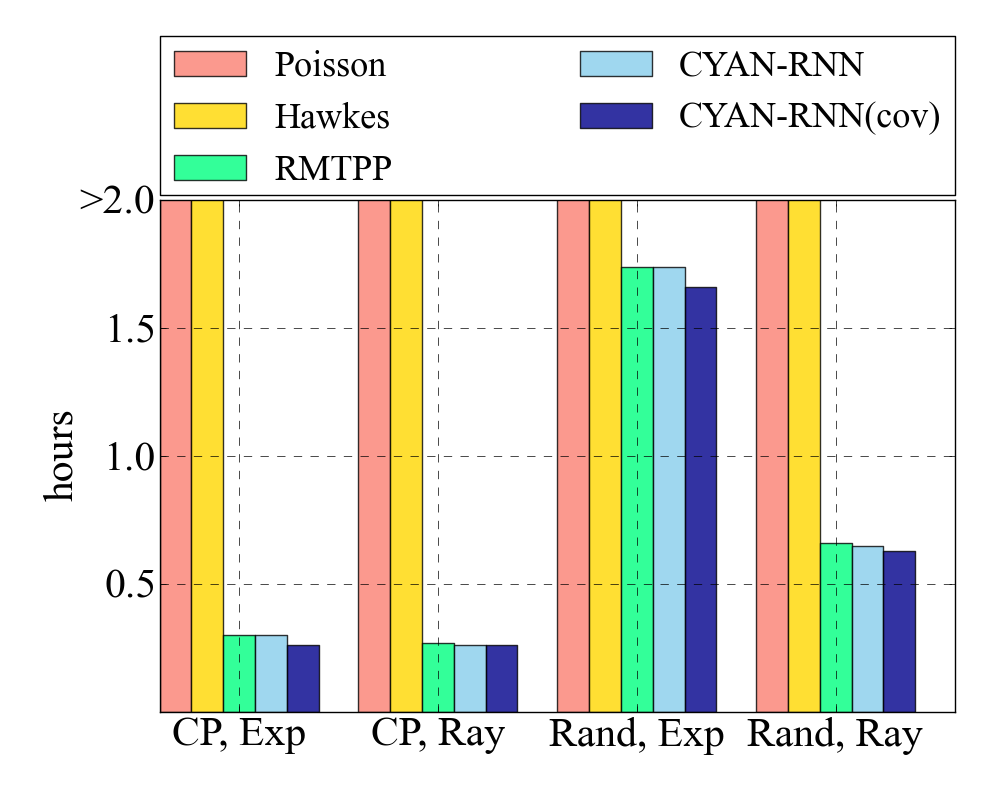
\includegraphics[width=0.35\textwidth]{figs/toy_rmse.png}
% }
% \caption{The next activated user and time predictions on real data. (a) The
% performance of predictions on next activated users related to baselines and our
% proposed models; (b) The performance of predictions on next activated time
% related to baselines and our proposed models.}
% \end{figure}

% \noindent{\textbf{Visualization.}} 
